\chapter{Testy}
\label{chapter-5}
\section{Konfiguracja}
Dla celów testów przyjęto pewne sztywne założenia. Wszystkie testy są przeprowadzane na sygnałach mowy próbkowanych na częstotliwości 4kHz. STFT i ISTFT jest obliczane przy pomocy okna hanninga \cite{hann} ze współczynnikiem nachodzenia okien(ang. overlap) 50$\%$. Jako okno przestrzenne wspomniane w \ref{alg:gprim} także przyjęto okno hanninga o szerokości $20^{\circ}$. Współczynniki $\alpha_{\mathrm{LT}}$ i $\alpha_{G}$ mają wartości 0.9. Jako macierz mikrofonową przyjęto kwadratową strukturę o liczbie mikrofonów $M=16$ o równomiernej odegłości między mikrofonami równej $\delta d = 1cm$. Na potrzeby niektórych eksperymentów odległość między mikrofonami była zwiększana.

\begin{figure}[h!]
    \centering
    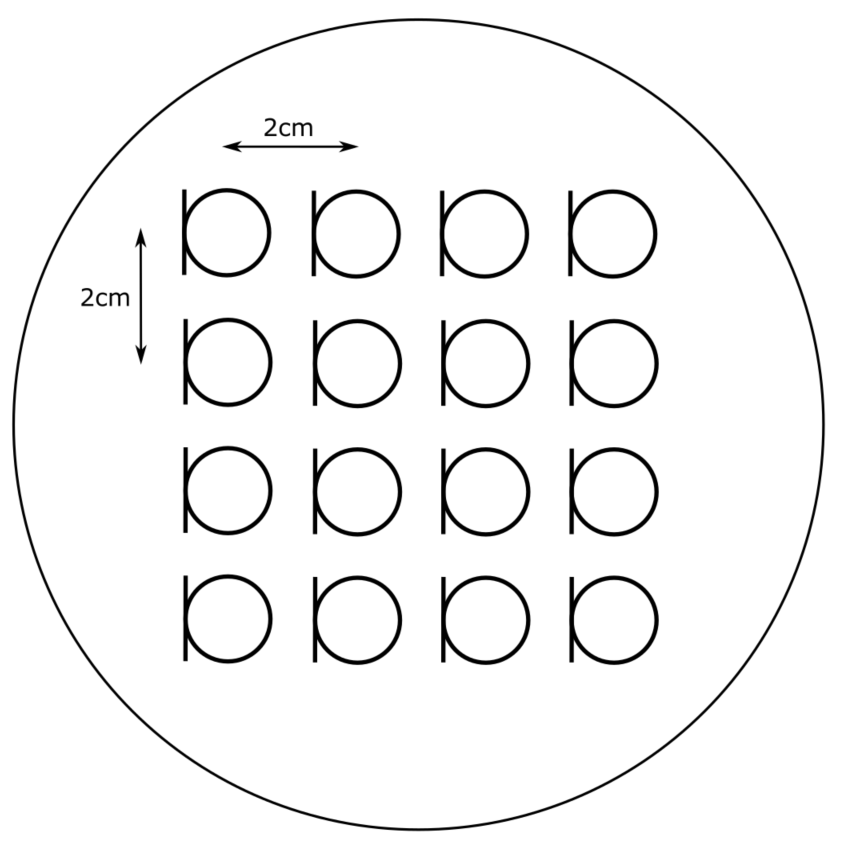
\includegraphics[width=0.4\textwidth]{Images/microphone.png}
    \caption{Macierz Mikrofonowa}
    \label{fig:microphone}
\end{figure}

Jako zakłócenie do usunięcia wybrano biały szum. Jego macierz PSD może być zapisana jako:

W sekcjach poniżej kolejno opisywane są wykonywane testy i doświadczenia.

\section{Charakterystyka kierunkowa filtra LCMV}

Poniżej przedstawiono wykresy charakterystyki kierunkowej dla filtra LCMV o następujących parametrach:

\begin{itemize}
    \item $\theta_{0}=30^{\circle},\theta_{1}=120^{\circle},
    \theta_{2}=300^{\circle}$
    \item $G(\theta_{0})=4,G(\theta_{1})=2,G(\theta_{2})=1$
\end{itemize}

